\documentclass[compress,10pt,aspectratio=169]{beamer}

%%%%%%%%%%%%%%%%%%%%%%%
% Thème beamer ONERA :
% Options :
%%%%%%%%%%%%%%%%%%%%%%%
%     - english -> biblio en anglais [défaut en français]
%	  (se sert de la mise en forme bibliographique onera.bst de Frédéric Cassaing (Frederic.Cassaing@onera.fr)
%	  (+url de la page de remerciement renvoie vers le site ONERA en anglais [défaut renvoie sur le site en français]).
%     - customnumbering -> permet d'afficher la numérotation des diapositives de manière élégante.
%	  (/!\ la compilation peut être longue avec cette option si il y a beaucoup de diapositives ! Il vaut mieux alors compiler sans l'option
%	   puis compiler une fois les diapositives finalisées).
%     - DR, CD, SD, S, TS -> ajout de la mention 'DIFFUSION RESTREINTE' ou 'CONFIDENTIEL DEFENSE' ou 'SECRET DEFENSE' ou 'SECRET' ou 'TRES SECRET'(rouge) dans le footer de la présentation. (Note, il ne faut choisir qu'une seule mention à la fois!)
%     - SF -> ajout de la mention 'SPECIAL FRANCE' (bleu) dans le footer de la présentation
\usetheme[customnumbering]{onera}
%\usetheme[english]{onera}


%%%%%%%%%%%%%%%%%%%%%%%
% Packages additionnels
%%%%%%%%%%%%%%%%%%%%%%%
\usepackage{amsmath,amssymb,amsfonts}
\usepackage{stmaryrd}
\usepackage{multirow}
\usepackage{bbold}
\usepackage{epsfig}
\usepackage{ulem}
\usepackage{comment}
\newcommand{\thicktilde}[1]{\mathbf{\tilde{\text{$#1$}}}}


\usepackage{algorithm2e}
\renewcommand{\listalgorithmcfname}{Liste des Algorithmes}%
\renewcommand{\algorithmcfname}{Algorithme}%
\renewcommand{\algorithmautorefname}{algorithme}%
\renewcommand{\algorithmcflinename}{ligne}%
%\renewcommand{\algocf@typo}{\ }%
%\renewcommand{\@algocf@procname}{Proc\'edure}%
%\renewcommand{\@algocf@funcname}{Fonction}%
\renewcommand{\procedureautorefname}{proc\'edure}%
\renewcommand{\functionautorefname}{fonction}%
%\renewcommand{\algocf@languagechoosen}{french}%

%\SetKwHangingKw{HDonnees}{Donnees$\rightarrow$}
%\SetKwInpsut{Donnees}{Donn\'ees}%
%\SetKwInput{Res}{R\'esultat}%
\SetKwInput{Entrees}{Entr\'ees}%
\SetKwInput{Entree}{Entr\'ees}%
\SetKwInput{Sortie}{Sortie}%
\SetKwInput{Sorties}{Sorties}%
%\SetKw{KwA}{\`a}%
%\SetKw{Retour}{retourner}%
%\SetKwBlock{Deb}{d\'ebut}{fin}%
\SetKwRepeat{Repeter}{r\'ep\'eter}{jusqu'\`a}%
%
\SetKwIF{Si}{SinonSi}{Sinon}{si}{alors}{sinon si}{sinon}{fin si}%
\SetKwSwitch{Suivant}{Cas}{Autre}{suivant}{faire}{cas o\`u}{autres cas}{fin cas}{fin d'alternative}%
\SetKwFor{Pour}{pour}{faire}{fin pour}%
\SetKwFor{PourPar}{pour}{faire en parall\`ele}{fin pour}%
\SetKwFor{PourCh}{pour chaque}{faire}{fin pour chaque}%
\SetKwFor{PourTous}{pour tous}{faire}{fin pour tous}%
\SetKwFor{Tq}{tant que}{faire}{fin tq}%


% Dessin (Note : le package 'tikz' est chargé par défaut avec le thème ONERA ainsi que l'option 'positioning')
\usepackage{tikz-3dplot}
\usetikzlibrary{shapes.misc}
\tikzset{cross/.style={cross out, draw=black, fill=none, minimum size=2*(#1-\pgflinewidth), inner sep=0pt, outer sep=0pt}, cross/.default={2pt}}

%%%%%%%%%%%%%%%%%%%%%%%
% Définition de la page de titre %%%%%  A COMPLETER OU IL Y A DEJA DU TEXTE !!!   %%%%%%
%%%%%%%%%%%%%%%%%%%%%%%

%\title[]{Audition pour le poste d'ingénieur de recherches en mathématiques appliquées à l'ONERA\vspace{0.5cm}}

%\subtitle[]{Kokou Michaelis Dotse\vspace{0.5cm}}
%\author[]{Kokou Dotse}\\
%*\href{mailto:kokou.dotse@onera.fr}{\texttt{kokou.dotse@onera.fr}}}
\date[]{}
%\directors{}
%\encadrant{}
%\encadrant{Vincent Mouysset(DTIS/MACI)\textsuperscript{1}}
%\grant{}
%\tutor{} % D'autres personnes importantes (DGA etc.)
%\institute{\inst{1}ONERA The French Aerospace Lab, Toulouse, France}
\logoUn{} %N'apparaît que si est rempli
\logoDeux{} %N'apparaît que si est rempli




%%%%%%%%%%%%%%%%%%%%%%%%%%%%%%%%%%%%%%%%%%
% Début du document
\begin{document}

% Page de titre (optionnel) %
%\MakeTitlePage

%\graphicspath{{../img//}}

%%%%%%%%%%%%%%%%%
% CORPS DE LA PRESENTATION %
%%%%%%%%%%%%%%%%%


\begin{frame}[plain]
\centering
\Large
\textbf{\color{onera}Audition pour le poste d'ingénieur de recherches en mathématiques appliquées à l'ONERA}\\
\vspace{1cm}
\textbf{\color{onera_gray}Kokou Michaelis Dotse}\\
\vspace{1cm}
\normalsize
08/07/2024
\end{frame}


\begin{frame}{Plan}
%\tableofcontents
\vspace{-0.4cm}
\begin{enumerate}
    \item \color{onera} Cursus et expériences professionnelles\\\vspace{0.5cm}
    \item Travaux de recherche \\\vspace{0.5cm}
    \item Projet de recherche et intégration dans les activités de MACI/ONERA\\\vspace{0.5cm}
    \item Conclusion
\end{enumerate}
\end{frame}



\begin{frame}{Cursus et expériences professionnelles}
\small
%\vspace{-0.3cm}
\begin{itemize}
\item {\color{onera} Licence en mathématiques (2012-2015):} Faculté des sciences, Université de Lomé, Togo. {\color{onera_gray} Licence classique, générale de mathématique, opportunité.}\\\vspace{0.8cm}

\item {\color{onera} Mastrer 1 et 2 en mathématiques fondamentales (2016-2018):} Institut de Mathématiques et de Sciences Physiques, Université d'Abomey Calavi, Bénin.\\
Mémoire: Utilisation des statistiques et du calcul parallèle pour faire de l’adaptation de maillage sous la supervision de Frédéric Hecht (LJLL/Sorbonne Université). {\color{onera_gray} Génération de maillages aléatoires et utilisation de la dispersion des résultats comme indicateur d'erreur.}\\
Financé par une bourse d'excellence de la banque mondiale.\\
\vspace{0.3cm}
\end{itemize}
\end{frame}



\begin{frame}{Cursus et expériences professionnelles}
\small
\vspace{-0.2cm}
\begin{itemize}
\item {\color{onera} Master 2 en ingénierie mathématiques (2019-2020):} Sorbonne Université, France. financé par la Fondation Sciences Mathématiques de Paris (FSMP).\\
Stage: Génération de maillages quadrilatéraux par résolution numérique d’équations aux dérivées partielles effectué à l'ONERA sous la supervision de Vincent Mouysset et de Sébastien Pernet.\\
{\color{onera_gray} Etude et implémentation d'une méthode de génération de maillages quadrilatéraux basé sur les champs de croix.}\\\vspace{0.6cm}

\item {\color{onera} Doctorat en mathématiques appliquées (2020-2024):} ONERA, ISAE-SUPAERO, France.\\
Financé par l'ONERA et dirigé par Vincent Mouysset et Sébastien Pernet. \\
Création de maillages quadrilatéraux bloc structurés à partir de champ de croix prescrit et respectant les caractéristiques physiques d'une scène de calcul.\\
{\color{onera_gray} Mise en place d'un cadre théorique et discret permettant la génération de maillages quadrilatéraux à partir de champs de croix arbitraires.}\\\vspace{0.2cm}
\end{itemize}
\end{frame}


\begin{frame}{Cursus et expériences professionnelles}
\small
\vspace{-0.2cm}
\begin{itemize}

\item {\color{onera}Encadrement d'un stage (Juin 2022/Août 2022)} avec Vincent Mouysset.\\
Comparaison de performances de schémas Galerkin discontinus définis sur maillages en triangles et en quadrangles.\\
{\color{onera_gray}Tristan Portugues de l'Institut National des Sciences Appliquées (INSA) de Toulouse.}\\\vspace{0.3cm}

\item  {\color{onera}Travaux dirigés et travaux pratiques} (Université Paul Sabatier et ISAE-SUPAERO): analyse numérique, théorie des EDP et méthodes numériques, méthodes numériques\\\vspace{0.3cm}


\item {\color{onera} Attaché temporaire d'enseignement et de recherche (2023-2024): } Faculté des Sciences et Ingénierie, Université Paul Sabatier.\\
198 heures de cours, travaux dirigés et travaux pratiques en Licence et en Master: {\color{onera_gray}Intégration et séries numériques, Algorithmique et calcul scientifique, Ensembles 2, Calcul différentiel et équations différentielles, Fonctions et calculs 3, Intégration et séries numériques, Analyse de Fourier et théorie du signal, Modélisation.}\\\vspace{0.2cm}
\end{itemize}
\end{frame}

\begin{frame}{Plan}
%\tableofcontents
\vspace{-0.4cm}
\begin{enumerate}
\color{onera}
\item {\color{onera_gray}Cursus et expériences professionnelles}\\\vspace{0.5cm}
\item {\color{onera}Travaux de recherche} {\small \color{black}(Création de maillages quadrilatéraux bloc structurés à partir de champ de croix prescrit et respectant les caractéristiques physiques d'une scène de calcul)} \\\vspace{0.5cm}
\item {\color{onera_gray}Projet de recherche et intégration dans les activités de MACI/ONERA}\\\vspace{0.5cm}
\item {\color{onera_gray}Conclusion}
\end{enumerate}
\end{frame}


\begin{frame}{Travaux de recherche}
\small
\begin{columns}
    \begin{column}{0.8\textwidth}
    \vspace{-0.3cm}
\begin{itemize}
\item {\color{onera} Le maillage :} discrétisation en cellules élémentaires, indispensable lors des simulations numériques (mécanique des fluides, électromagnétisme, etc.). Les maillages triangulaires ("mesh tri") sont bien développés depuis plus d'un demi-siècle. La génération de bons maillages quadrilatéraux ("mesh quad") reste complexe.\\\vspace{0.25cm}

\item {\color{onera} Maillages quadrilatéraux ("mesh quad") :} présentent d'excellentes propriétés pour plusieurs schémas (DF, FEM, DS, GD, etc.).\\\vspace{0.2cm}

\item {\color{onera} Structuré :} faible stockage, optimisé pour le calcul parallèle.\\\vspace{0.2cm}

\item {\color{onera} Nature tensorielle :} adapté à la montée en ordre, quadrature, systèmes creux.\\\vspace{0.2cm}

\item {\color{onera} Étirement anisotropique :} maillage de couche limite, capture des fortes variations.\\\vspace{0.25cm}
\end{itemize}
    \end{column}
    \begin{column}{0.24\textwidth}
        \centering
        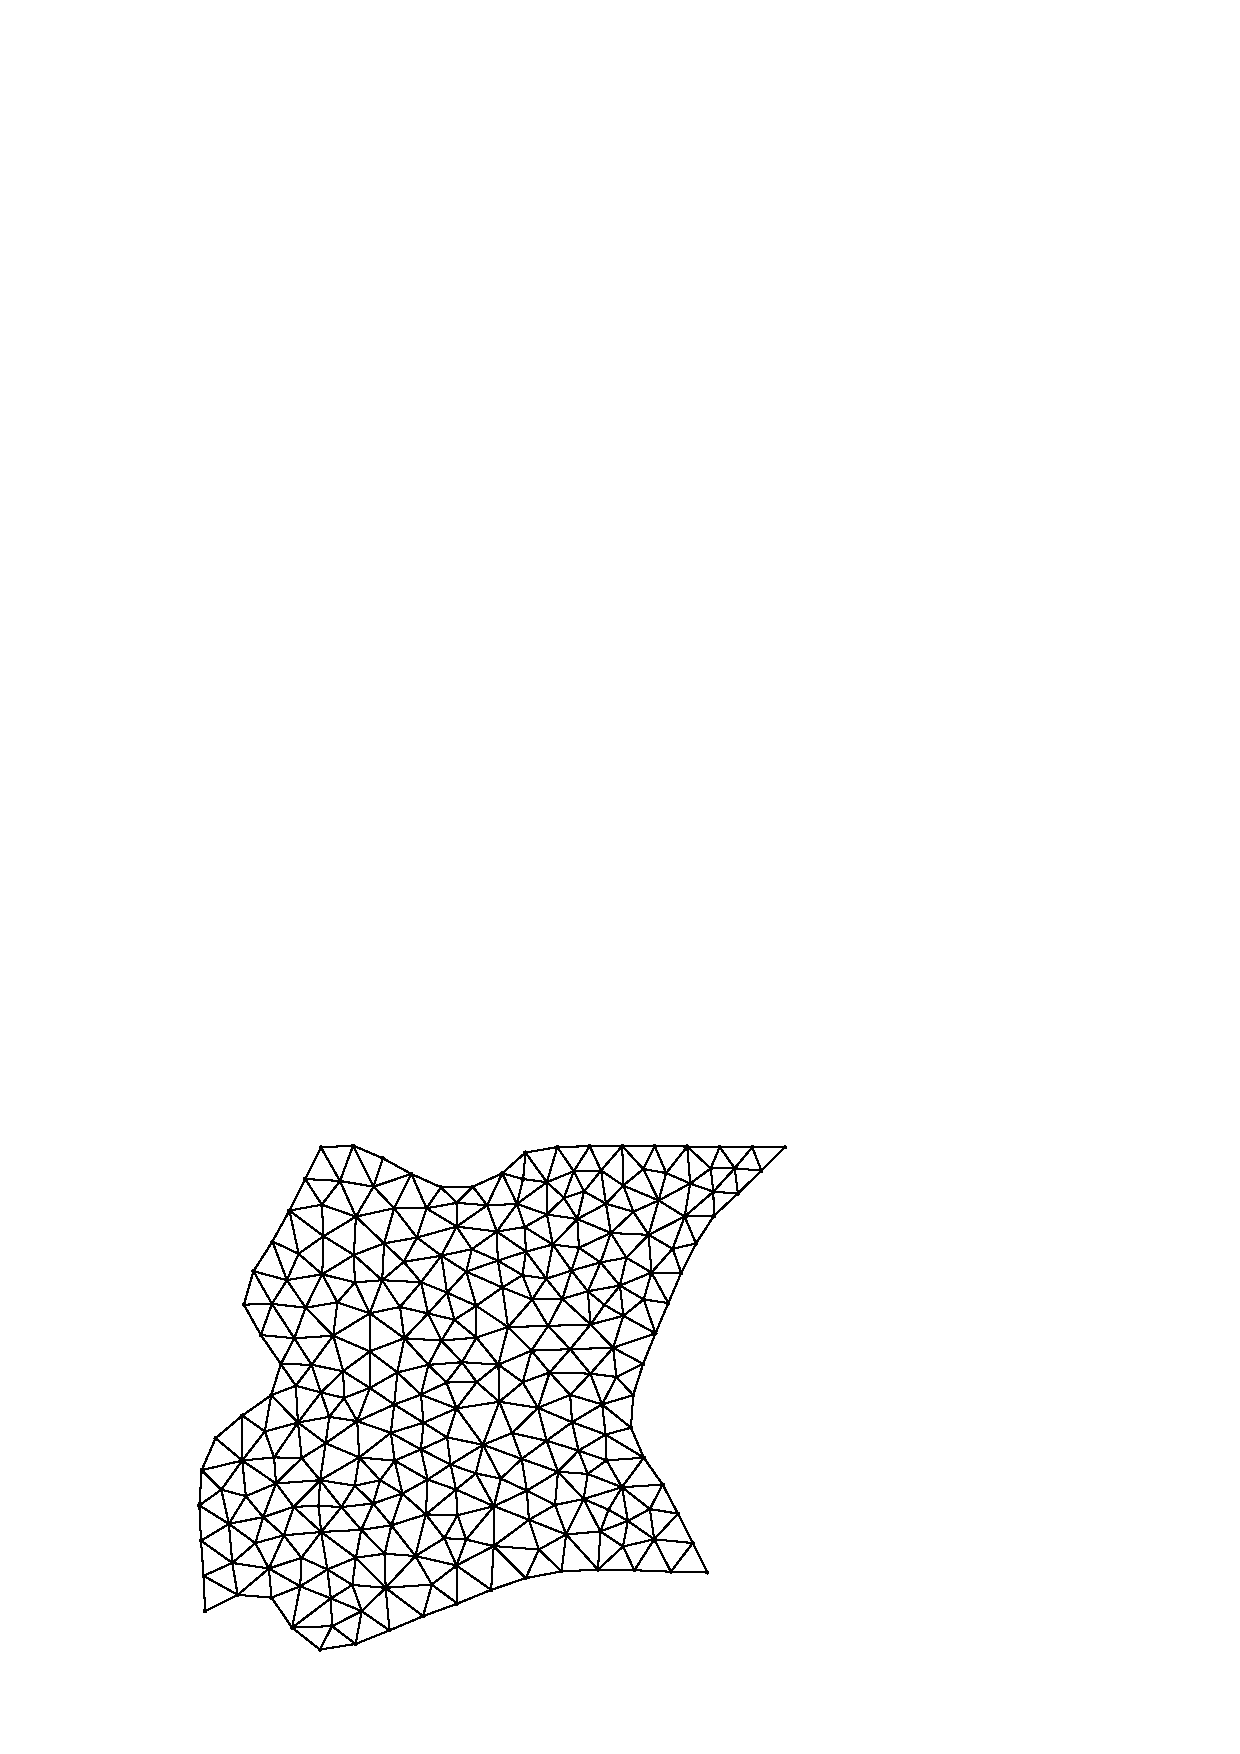
\includegraphics[scale=0.11]{images/zone4beamer.pdf}
        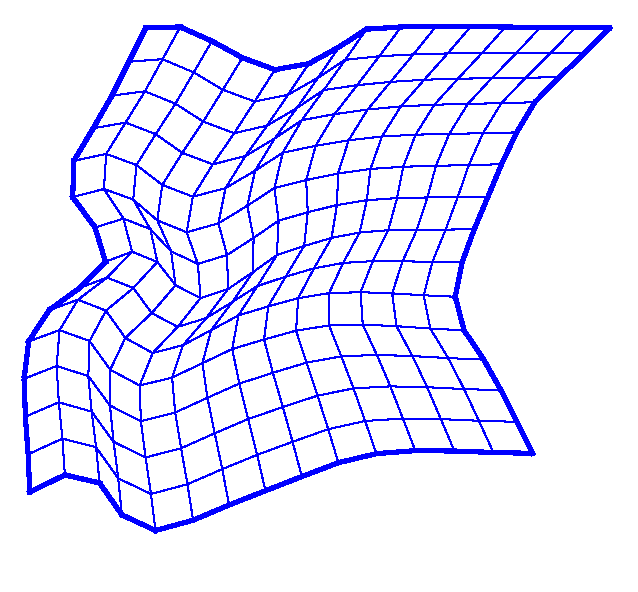
\includegraphics[scale=0.35]{images/mesh_zone4.eps}
    \end{column}
\end{columns}
\end{frame}

\begin{frame}{Travaux de recherche}
\small
\begin{columns}
    \begin{column}{0.7\textwidth}
        {\bf Quelques méthodes de génération de "Mesh quad".}\vspace{0.2cm}
        \begin{itemize}


\onslide<1->{
            \item {\color{onera} Blocs structurés manuels}\\\vspace{0.1cm}}

\onslide<2->{
            \item {\color{onera} Conversion Tri-to-quad:} subdivision de Catmull-Clark {\color{gray} [ E. Catmull, J. Clark (1978)]}, operation edge-flip {\color{onera_gray} [ MeshLab, SQuad, BlossomQuad (2011)]}, quads non-structuré.}\\\vspace{0.1cm}


\onslide<3->{
            \item {\color{onera} Méthodes de grille cartésienne:} intersection domaine-grille {\color{onera_gray} [Schneiders (1996)]}, génèrent des mailles de mauvaises qualités le long de la frontière}\\\vspace{0.1cm}


\onslide<4->{
            \item {\color{onera} Avancée de front:} pavage {\color{onera_gray}[D. Blacker, B. Stephenson (1991)]}, H-Morph {\color{onera_gray}[Owen et al (2000)]}.}\vspace{0.1cm}


%\onslide<5->{\item {\color{onera} Axe médian:} simplification de la géomtrie en identifiant un squelette central {\color{onera_gray}[Nackman and Srinivasan, 1989]}.}\vspace{0.1cm}

        \end{itemize}
    \end{column}


        \begin{column}{0.25
        \textwidth}
\centering
\only<2>{
\vspace{-0.15cm}
    \includegraphics[scale=0.22]{images/tri_to_quad_1_beam.png}
\vspace{0.2cm}
}
\only<3>{
%\vspace{-0.2cm}
    \includegraphics[scale=0.28]{images/superpo_grid_1_beam.pdf}
\vspace{0.18cm}
}
\only<4>{
%\vspace{-0.2cm}
    \includegraphics[scale=1]{images/front_advance_beam.pdf}
%\vspace{0.15cm}
}
%\only<4>{
%\vspace{-0.2cm}
    %\includegraphics[scale=0.13]{images/median_axis.pdf}
%\vspace{0.15cm}
%}
\end{column}
\end{columns}
\end{frame}

\begin{frame}{Travaux de recherche}{Une approche basée sur les champs de croix}
\small
\vspace{-0.2cm}
\begin{columns}
\begin{column}{0.25\textwidth}
\centering
%\onslide<1->{
\includegraphics[scale=0.068]{images/frey_1.pdf}\hspace{0.2cm}
\footnotesize Croix de bord
%}
\end{column}

\begin{column}{0.25\textwidth}
\centering
%\onslide<2->{
\includegraphics[scale=0.068]{images/frey_4.pdf}\hspace{0.2cm}
\footnotesize Champ de croix
%}
\end{column}

\begin{column}{0.25\textwidth}
\centering
%\onslide<3->{
\includegraphics[scale=0.068]{images/frey_5.pdf}\hspace{0.2cm}
\footnotesize Partitionnement
%}
\end{column}

\begin{column}{0.25\textwidth}
\centering
%\onslide<4->{
\includegraphics[scale=0.07]{images/frey_6.pdf}\vspace{0.05cm}
\footnotesize Maillage
%}
\end{column}
\end{columns}

\vspace{0.2cm}

\only<2->{

{\bf Avantages:}

%\vspace{0.15cm}

\begin{columns}

\begin{column}{0.5\textwidth}
\begin{itemize}
\item blocs structurés: {\color{onera_gray}faible stockage, connectivité efficace.}%, calcul parallèle.}
\item suivi de la frontière: {\color{onera_gray} fidèle à la CAO.}%, récupération automatique de la frontière.}
%\vspace{0.4cm}
\end{itemize}
\end{column}

\begin{column}{0.5\textwidth}
\begin{itemize}
\item qualités des éléments: {\color{onera_gray} topologiquement proche de carré, de rectangle, convexe.}
\item faible nombre de sommets irréguliers
%\vspace{0.4cm}
\end{itemize}
\end{column}
\end{columns}
\vspace{0.35cm}
Le respect simultané de toutes ces contraintes rend difficile la génération automatique de maillages quadrilatéraux.
}
\end{frame}


\begin{frame}{Travaux de recherche}{Une approche basée sur les champs de croix}
\small
\begin{columns}
    \begin{column}{0.55\textwidth}
    \only<1>{
    {\bf Les limites de cette approche:}\vspace{0.2cm}
        \begin{itemize}
            \item {\color{onera} Génération du champ de croix:} non-contrôle de la position des points singuliers, abscence de notion de point singulier de bord, non-homogénéité\vspace{0.2cm}
            \item {\color{onera} Domaine très étiré:} tend à produire des champs de croix contenant des points singuliers non isolés\vspace{0.2cm}
            \item {\color{onera} Analyse de la méthode:} approche Ginzburg-Landau, analyse complexe, {\color{onera_gray}[Viertel et al (2020)]}  \vspace{0.2cm}
            \item {\color{onera} Variété surfacique sans bords}
        \end{itemize}
    }

        \only<2>{
    {\bf Idée:} Mettre en place un processus permettant d'aboutir à des mesh quad à partir de champs de croix arbitraires\vspace{0.3cm}
        \begin{itemize}
            \item Choisir un champ de croix ayant des caractéristiques plus convenable \vspace{0.3cm}
            \item Analyse théorique de la méthode pour comprendre la formation des partitions à 4 côtés.
        \end{itemize}
    }

    \end{column}
    \begin{column}{0.45\textwidth}
        \centering
        \vspace{-0.15cm}
        \includegraphics[scale=0.12]{images/new_cercle.png}
        \hspace{0.6cm}
        \includegraphics[scale=0.28]{images/carreTrou.png}
        \\\vspace{0.2cm}
        \includegraphics[scale=0.18]{images/triangle_etire.png}
        \hspace{0.2cm}
        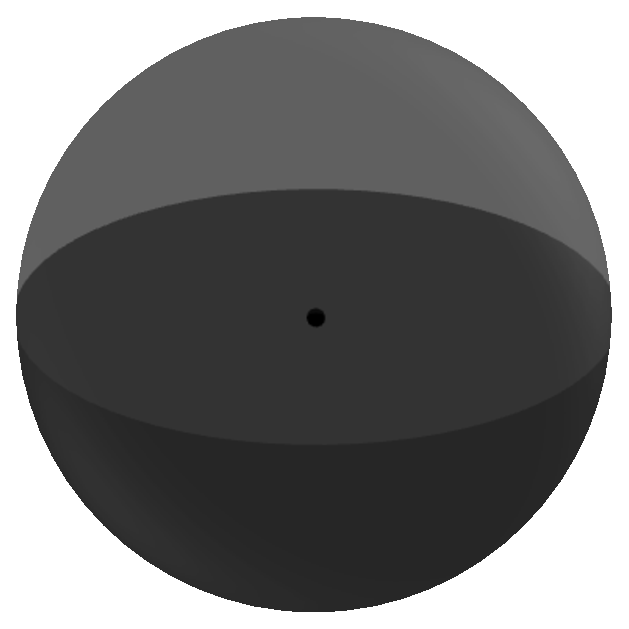
\includegraphics[scale=0.23]{images/sphere.eps}
        \vspace{0.3cm}
    \end{column}
\end{columns}
\end{frame}




\begin{frame}{Travaux de recherche}{Prise en compte de champs de croix arbitraires}
\small
Une {\color{onera}croix} est un élément de l'ensemble quotient $\mathbb{S}^1/\mathcal{Q}\cup\{0\}$ {\color{onera_gray}(cercle unité, ensemble de 4 vecteurs)}.\\\vspace{0.2cm}
Un {\color{onera}champ de croix} est une application $\bar{u}:p\in\Omega\rightarrow \bar{u}(p)\in S^1/\mathcal{Q}\cup\{0\}$.\\\vspace{0.2cm}

\begin{onerablock}[drop fuzzy shadow]{\small Définition}
\small
$\bar{u}$ est un champ de croix \emph{presque-$\mathcal{C}^1$} si $\bar{u}$ est de classe $\mathcal{C}^1$ en tout point sauf en un nombre fini de point {\color{onera_gray}(les points singuliers)}.
\end{onerablock}

{\bf\underline{Exemple:}} {\color{onera_gray} champ de croix à partir d'un mode propre du laplacien sur le demi-disque. Tangente et gradient des isolines. Pts. sing. et extrémas. Quart de l'angle des croix. Partitionnement. Outil.}



    \begin{columns}
        \begin{column}{0.33\textwidth}
        \centering
\onslide<2->{
        %\includegraphics[scale=0.091]{images/mode_prop.pdf}
        \includegraphics[scale=0.092]{images/mode_prop_new.pdf} \hspace{0.2cm}
        %\footnotesize Mode propre du laplacien sur le demi-disque
%        }
        \end{column}
        \begin{column}{0.33\textwidth}
        \centering
%\onslide<2->{
        \includegraphics[scale=0.092]{images/tang_grad.pdf} \hspace{0.2cm}
        %\footnotesize Tangentes aux lignes de niveaux
        }
        \end{column}
        \begin{column}{0.33\textwidth}
        \centering
\only<3>{
        \includegraphics[scale=0.092]{images/mode_prop_cross_beam.pdf} \hspace{0.2cm}
        %\footnotesize Champ de croix
        }
\only<4>{
        \includegraphics[scale=0.092]{images/mode_prop_stream_non_align_beam.pdf} \hspace{0.2cm}
        %\footnotesize Champ de croix
        }
        \end{column}
    \end{columns}
\end{frame}



\begin{frame}{Travaux de recherche}
\small
\vspace{-0.2cm}
  \begin{columns}
    \begin{column}{0.7\textwidth}
{\bf Qu'est ce qu'une partition de quatres côtés ?}\\\vspace{0.2cm}
    {\color{onera} Index:} nombre d'enroulement du champ autour d'un point
\begin{itemize}
    \item si $p\in\Omega$ alors $id_{\bar{u}}(p) = \frac{1}{2\pi}\int_\gamma d\theta_{\bar{u}}$
    \item si $p\in\partial\Omega$ alors $id^\partial_{\bar{u}}(p)=\frac{1}{2\pi}\left[\pi-\hat{p}+\lim\limits_{s\rightarrow 0}\int_s^{1-s}d\theta_{\bar{u}}^\gamma\right]$
\end{itemize}
{\color{onera} Valence:} nombre de séparatrices associé à un point
\begin{itemize}
    \item si $p\in\Omega$ alors $N_s(p) = 4-4id_{\bar{u}}(p)$
    \item si $p\in\partial\Omega$ alors $N_s(p) = 3-4id^\partial_{\bar{u}}(p)$
\end{itemize}
{\bf Exemple:} (Voir figure)\\\vspace{0.1cm}
\begin{onerablock}[drop fuzzy shadow]{\small  Lemme}
    \small L'index de bord d'un point (singulier ou d'intersection) par rapport à une partition $\mathcal{P}$ donnée est 1/4.
\end{onerablock}
    \end{column}
    \begin{column}{0.3\textwidth}
        \centering
  \includegraphics[scale=0.1]{images/sepa_3.pdf}
  \scriptsize $id_{\bar{u}}(p)=1/4, N_s(p) = 3$
  \\\vspace{0.1cm}
  \includegraphics[scale=0.1]{images/sepa_5.pdf}
  \scriptsize $id_{\bar{u}}(p)=-1/4, N_s(p) = 5$
  \\\vspace{0.3cm}
    \end{column}
\end{columns}

\end{frame}

\begin{frame}{Travaux de recherche}
\small
%{\bf Qu'est ce qu'une partition de quatres côtés ?}\\
\vspace{-0.2cm}
On exploite ce résultat de la manière suivante: {\color{onera_gray} (formation des partition de 4 côtés)}\\\vspace{0.1cm}
 Soit $\mathcal{P}$ une partition quelconque. {\color{onera_gray} (A cette étape on ne connait pas encore son nombre côtés, séparatrice à l'aveugle)}
$$\chi(\mathcal{P})=1. \quad\quad{\color{onera_gray} (\chi=2-2g-b, g=0, b=1)}$$
Par construction, les bords de la partition sont aligné avec le champ et elle ne contient pas de points singulier interne). Le théorème de Poincaré-Hopf donne alors:
$$\chi(\mathcal{P})=\sum_{i=1}^{n_c}id_{\bar{u}}(c_i).$$
Par combinaison, on obtient:
$$1=\sum_{i=1}^{n_c}\frac{1}{4}\Longrightarrow n_c=4.$$
\textbf{Conclusion :} Toute partition dont le bord est aligné avec le champ (séparatrices) aura 4 côtés.
\vspace{0.4cm}
\end{frame}



\begin{frame}{Travaux de recherche}{Un exemple de champ de croix alignés sur le bord du domaine}

    \begin{columns}
        \begin{column}{0.33\textwidth}
        \centering
        \includegraphics[scale=0.087]{images/demi_disc_align_first.pdf} \hspace{0.2cm}
        \footnotesize Champ de croix
        \end{column}
        \begin{column}{0.33\textwidth}
        \centering
        \includegraphics[scale=0.087]{images/demi_disc_align_second.pdf} \hspace{0.2cm}
        \footnotesize Partitionnement
        \end{column}
        \begin{column}{0.33\textwidth}
        \centering
        \includegraphics[scale=0.087]{images/demi_disc_align_third.pdf} \hspace{0.2cm}
        \footnotesize Maillage
        \end{column}
    \end{columns}
    \vspace{0.4cm}
        \begin{onerablock}[drop fuzzy shadow]{\small Théorème 1}
    \small
Soit $\Omega$ un domaine borné et fermé dans $\mathbb{R}^2$ avec une frontière régulière par morceau et soit $\bar{u}$ un champ de croix presque-$\mathcal{C}^1$ aligné avec $\partial\Omega$ tel que $0<Card(\mathcal{S}_{\bar{u}})<\infty$ et pour tout $p\in\Omega$, $id_{\bar{u}}(p)=k/4$ où $k\in\mathbb{Z}$ et $k\leq 1$. Si les séparatrices de $\bar{u}$ convergent alors le partitionnement résultant est une décomposition de $\Omega$ en régions à quatre côtés.
    \end{onerablock}
\end{frame}


\begin{frame}{Travaux de recherche}{Processus d'alignement}

\vspace{-0.3cm}
    \small
    \begin{columns}
    \begin{column}{0.7\textwidth}

\onslide<2->{
\textbf{Idée}: Mise en place d'un processus d'alignement par rotation des croix du bord pour les aligner avec la normale sortante, transformation globale et lisse du champ pour ne pas introduire de singularités.%{\color{onera_gray}( Proposition)}
\\\vspace{0.12cm}
}

\onslide<3->{

\begin{onerablock}[drop fuzzy shadow]{\small Proposition}
    \small
    Soit $\bar{u}$ un champ de croix presque-$\mathcal{C}^1$ sur $\Omega$ et $\theta:\Omega \rightarrow \mathbb{R}$ une fonction de classe $\mathcal{C}^1$ sur $\Omega$, alors $\bar{v}={\mathbf{R}(\theta)\bar{u}}$ est un champ de croix presque-$\mathcal{C}^1$ et pour tout $p\in \Omega\backslash\partial\Omega,~id_{\bar{u}}(p)=id_{\mathbf{R}(\theta)\bar{u}}(p)$.
    \end{onerablock}
    %{\color{onera_gray}(Conservation de certaines propriétés de $\bar{u}$)}\\\vspace{0.12cm}
    {\bf Diffusion de la différence angulaire entre $\bar{u}$ et $\bar{n}$:}
}

\vspace{0.1cm}

\onslide<3->{
%\vspace{0.4cm}
    \begin{equation*}
    \left\{
    \begin{array}{lcll}
    \Delta\phi &=& 0 &\mbox{ dans }\Omega,\\[0.3cm]
    \phi(p) &=& \widehat{(\bar{n}(p); \bar{u}(p))}=\theta_{\bar{n}}(p)-\theta_{\bar{u}}(p)&\mbox{ sur } \partial\Omega.
    \end{array}
    \right.
    \end{equation*}
    {\color{onera_gray}(Angle multivarié, defaut de régularité de $\phi$ et intro. sing. bord, chang. cond. bord.)}\\\vspace{0.12cm}
}


\end{column}

\begin{column}{0.32\textwidth}
        \centering
        \includegraphics[scale=0.09]{images/mode_prop_stream_non_align_beam.pdf}
        \only<1>{
        \footnotesize {\color{onera_gray}(Le bord ne fait pas partie des séparatrices. Champ de croix non aligné avec le bord du domaine.)}
        }
    \end{column}
    \end{columns}
\end{frame}

\begin{frame}{Travaux de recherche}{Processus d'alignement}
\small
\vspace{-0.4cm}
On se donne une paramétrisation \(\gamma\) sur \([0, 1]\) de \(\partial\Omega\).\\\vspace{0.12cm}
\(\theta_{\bar{u}}^\gamma\) et \(\theta_{\bar{n}}^\gamma\) sont des relèvements continus de \(\theta_{\bar{u}}\) et \(\theta_{\bar{n}}\) le long de \(\gamma\).\\\vspace{0.12cm}
\textbf{But} : Lisser l'angle en contrôlant l'emplacement des singularités dues à la non-périodicité des relèvements. L'équation d'alignement devient :\\\vspace{0.12cm}

\begin{equation*}
\left\{
\begin{array}{lcll}
\Delta\phi &=& 0 &\mbox{ dans } \Omega,\\[0.4cm]
\phi(\gamma(t)) &=& \theta_{\bar{n}}^\gamma(t) + \mathcal{I}(t) - \theta_{\bar{u}}^\gamma(t) & \mbox{ sur } \gamma^{-1}(\partial\Omega \backslash (\mathcal{B} \cup \mathcal{S}_{\bar{n}} \cup \mathcal{S}_{\bar{u}})).
\end{array}
\right.
\end{equation*}

\begin{equation*}
\mathcal{I}(t) = \sum_{s \in \gamma^{-1}(\mathcal{B} \cup \mathcal{S}_{\bar{n}})} \left[\underbrace{\left(\pi - \widehat{\gamma(s)}\right)}_{\text{courbure géodésique}} - \underbrace{\left(\lim\limits_{r \rightarrow s^+}\theta^{\gamma}_{\bar{n}}(r) - \lim\limits_{r \rightarrow s^-}\theta^{\gamma}_{\bar{n}}(r)\right)}_{\text{saut de }\bar{n}} - \underbrace{2\pi I_{\gamma(s)}}_{\text{index des pts. de }\mathcal{B}\text{( les coins)}}\right] \mathbb{1}_{[0, t]}(s).
\end{equation*}

On récupère ainsi une régularité \(\mathcal{C}^1\) par morceaux où les sauts sont localisés aux points de l'ens. \(\mathcal{B}\).

\end{frame}


\begin{frame}{Travaux de recherche}{Processus d'alignement}
\vspace{-0.2cm}
\small
En généralisant le théorème de Poincarré-Hopf au bord du domaine,
\begin{equation*}
\sum_{s\in Int(\Omega)} id_{\bar{v}}(s)+{\bf \color{red}\sum_{c\in \partial\Omega} id_{\bar{v}}(c)} = \chi(\Omega),
\label{poincareformula_3}
\end{equation*}

on dégage une contrainte générale sur le champ de croix "input":
\begin{equation*}
deg(\bar{u}, \partial\Omega) =\sum_{s\in Int(\Omega)} id_{\bar{u}}(s) = \sum_{s\in Int(\Omega)} id_{\bar{v}}(s) = \chi(\Omega)-\sum_{c\in \partial \Omega} id_{\bar{v}}(c).
\label{third_u_c}
\end{equation*}
\begin{onerablock}[drop fuzzy shadow]{Théorème 2}
Soit $\bar{u}$ un champ de croix tel que pour tout $p\in\Omega\backslash\partial\Omega$, ${\bf id_{\bar{u}}(p)<=1/4}$. \'Etant $\bar{u}$ donné un ensemble $(c_i)_{i\in\{1,\dots,n_b\}}\subset\partial\Omega$ de points distincts tel que:
$
{\bf deg(\bar{u}, \partial\Omega) = \chi(\Omega)-\sum_{i=1}^{n_b} id_{\bar{u}}(c_i),}
$
il existe un champ de croix $\bar{v}$ aligné sur le bord de $\Omega$ et vérifie le Théorème 1.
\end{onerablock}
\vspace{0.1cm}
{\bf Exemple:} Champ de croix construit à partir du mode propre du laplacien sur le demi disque.
\end{frame}


\begin{frame}%{\fontsize{12}{12}\selectfont Exemples}
\vspace{-0.28cm}
\begin{columns}
\begin{column}{0.4\textwidth}
    \centering
    \scriptsize
    $\chi(\Omega)=1$\\\vspace{0.1cm}
    $deg(\bar{u}, \partial\Omega) = 1/4+1/4$\\\vspace{0.1cm}
    $\sum_{i=1}^{2} id_{\bar{u}}(c_i)=1/4+1/4$\\\vspace{0.1cm}
    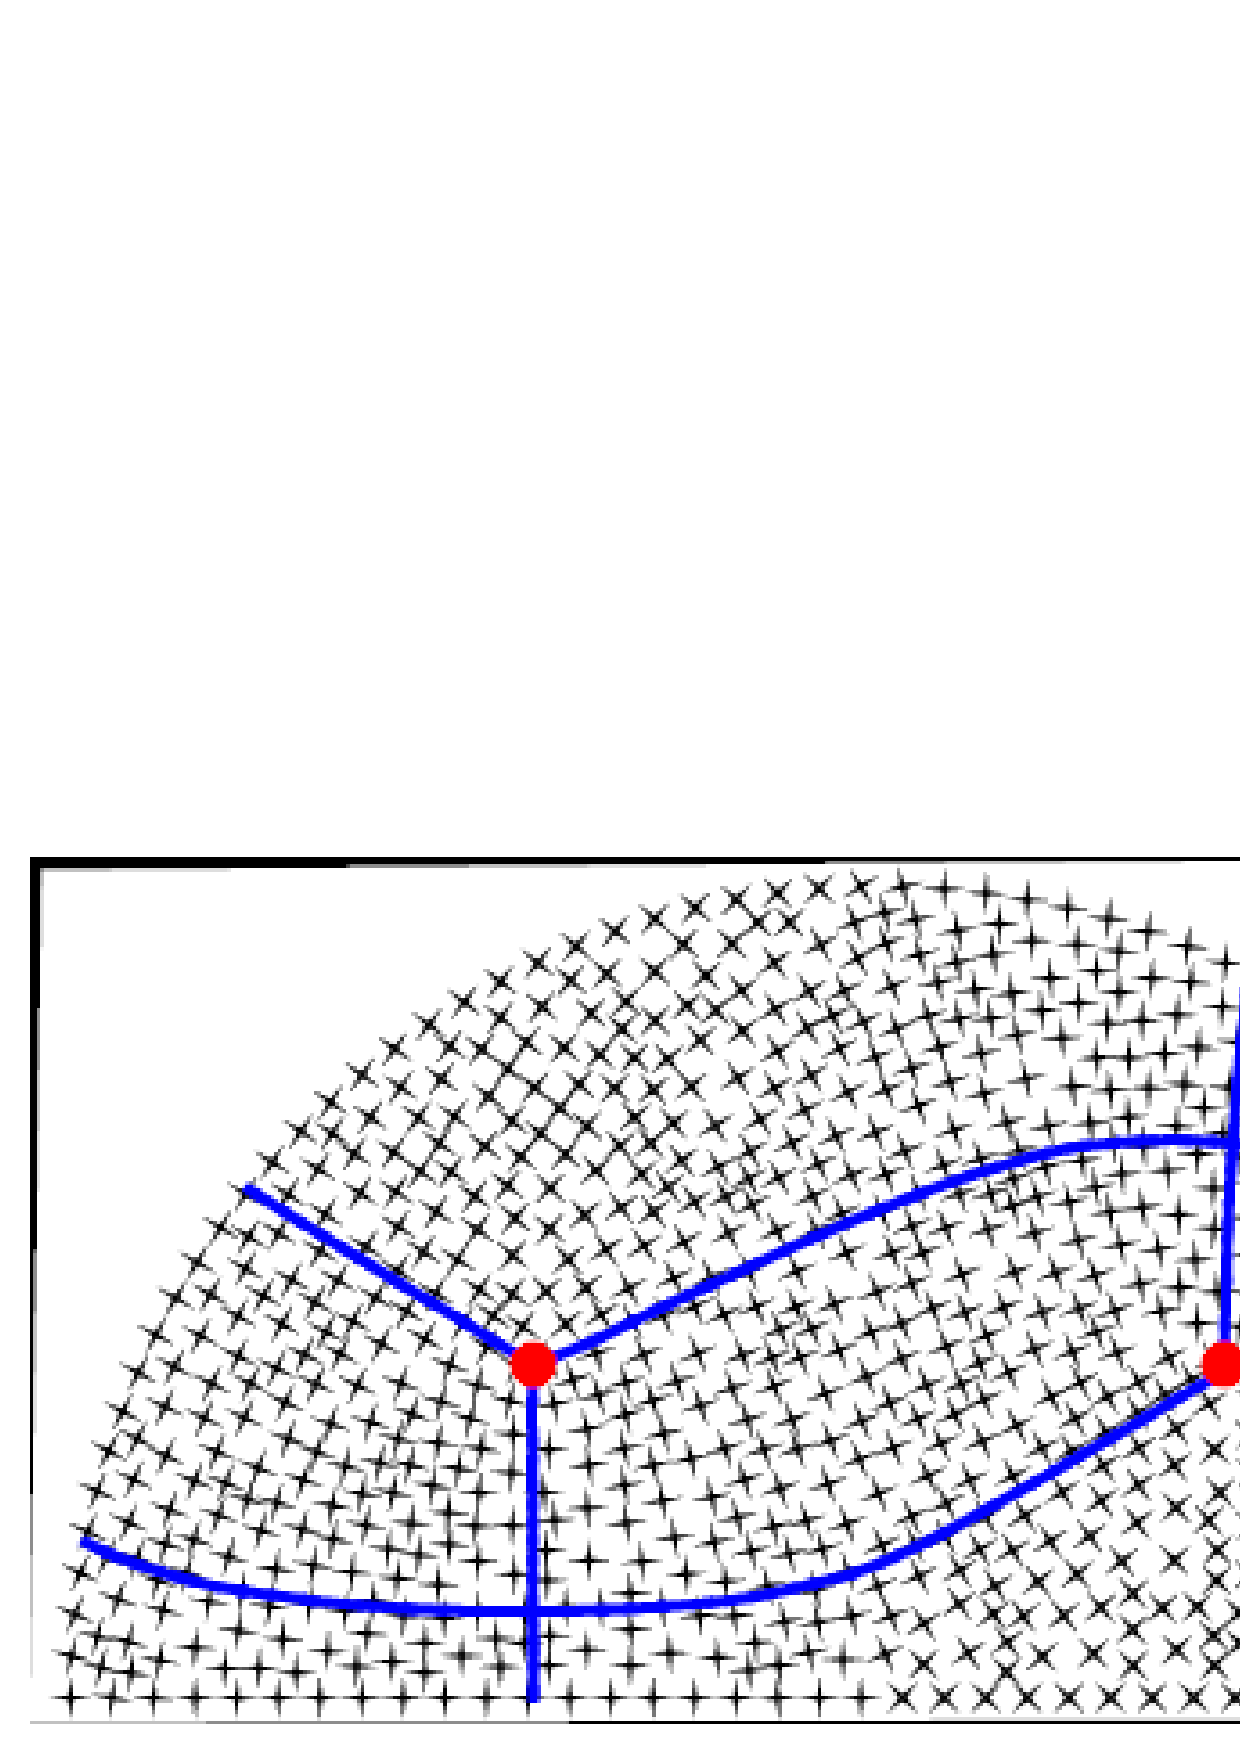
\includegraphics[scale=0.32]{images/demiDiscValPropNonAligne.pdf}\\\vspace{0.1cm}
    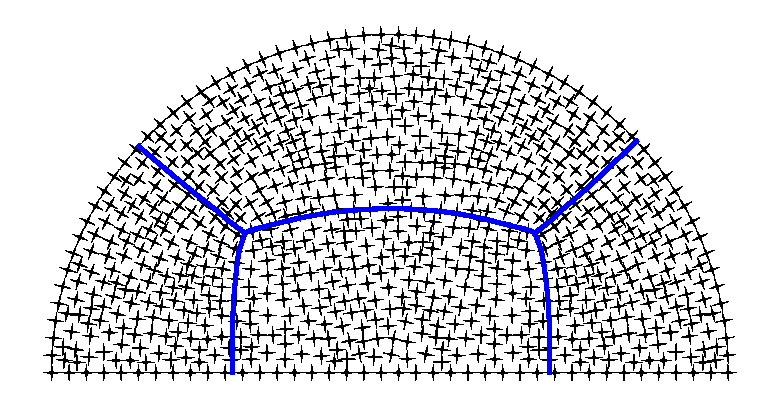
\includegraphics[scale=0.32]{images/demiDiscValPropAligne.eps}\\\vspace{0.1cm}
    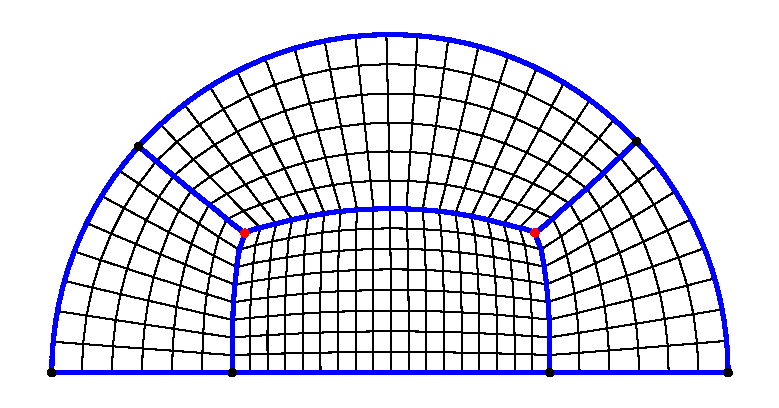
\includegraphics[scale=0.32]{images/mailDemiDisc.eps}\\
    \scriptsize {\color{onera_gray}(Mode propre)}
\end{column}
\pause
\begin{column}{0.4\textwidth}
    \centering
    \scriptsize
    $\chi(\Omega)=1$\\\vspace{0.1cm}
    $deg(\bar{u}, \partial\Omega) = 1/4+1/4$\\\vspace{0.1cm}
    $\sum_{i=1}^{2} id_{\bar{u}}(c_i)=1/4+1/4$\\\vspace{0.1cm}
    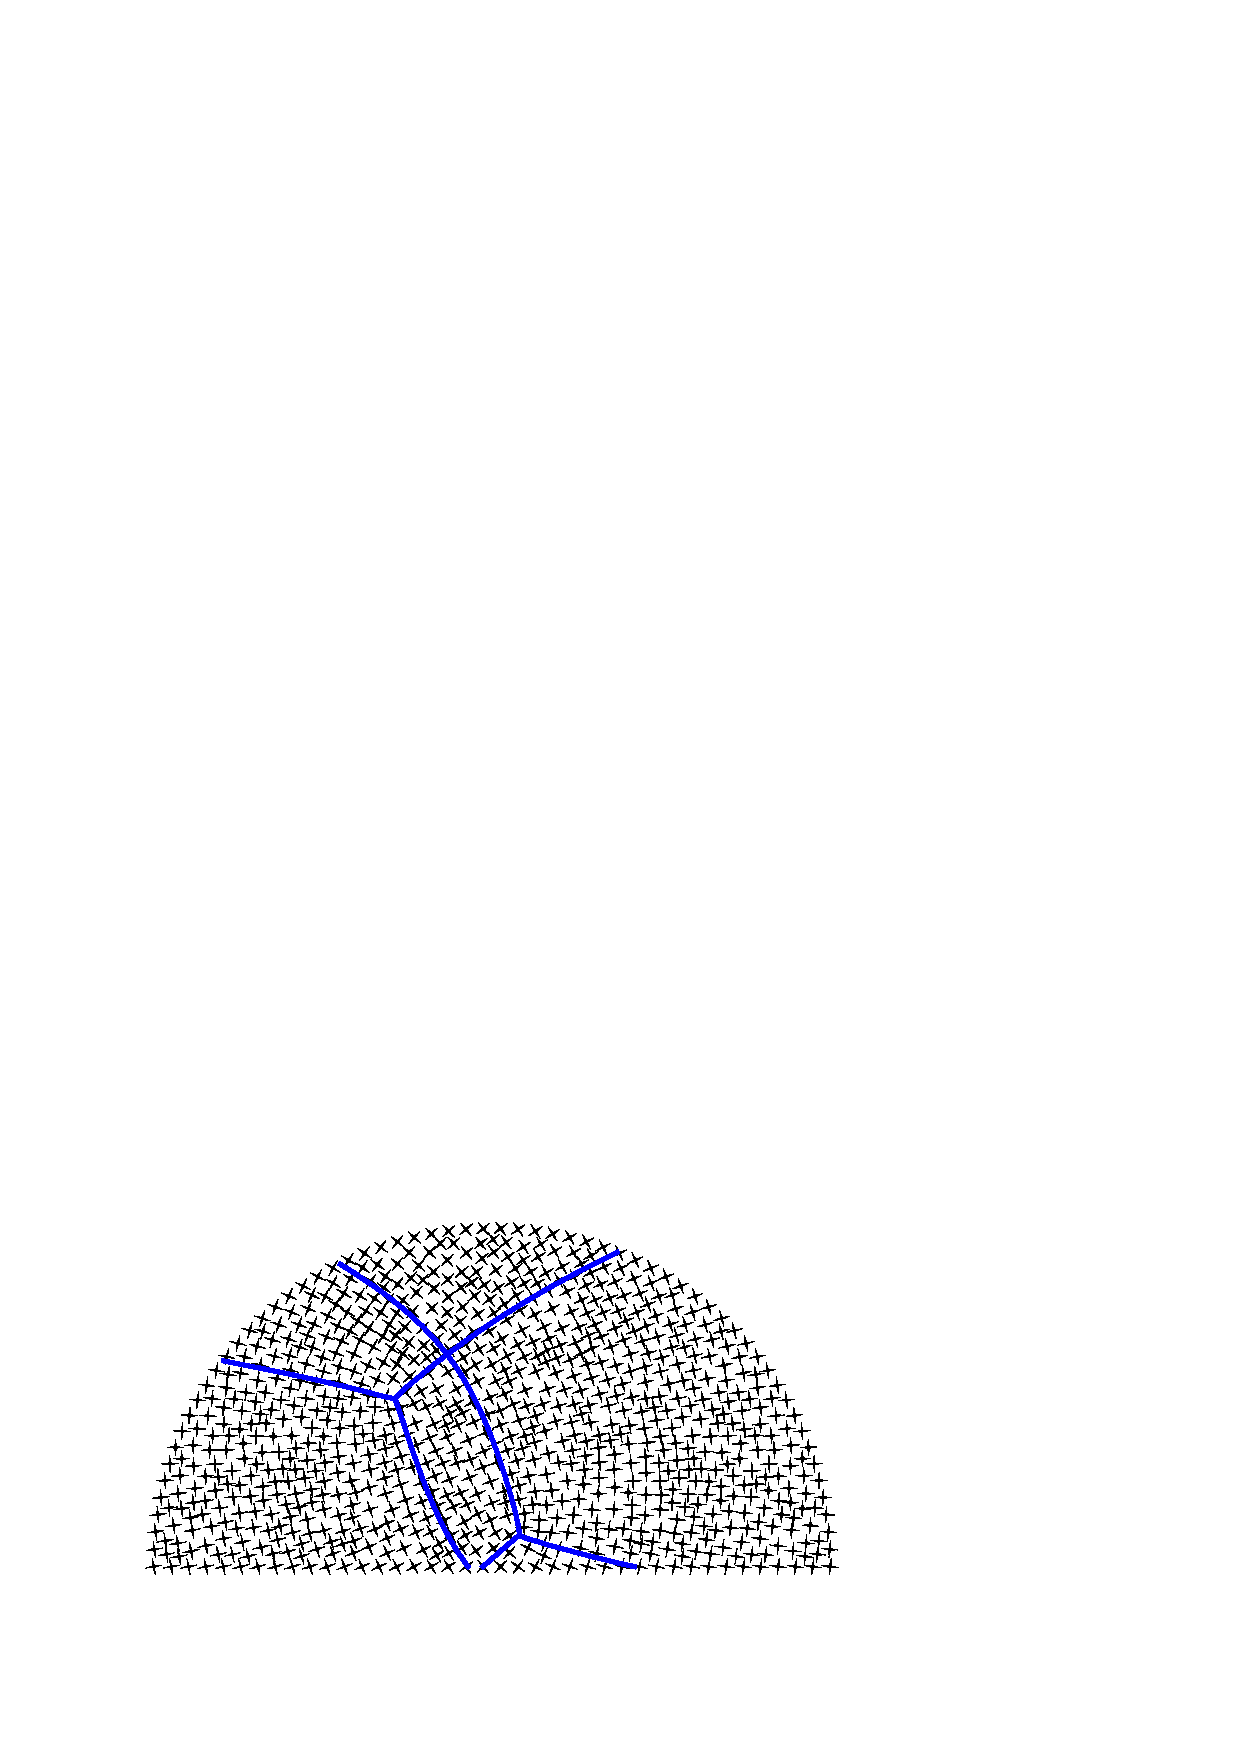
\includegraphics[scale=0.32]{images/demiDiscGinzNonAligne.pdf}\\\vspace{0.1cm}
    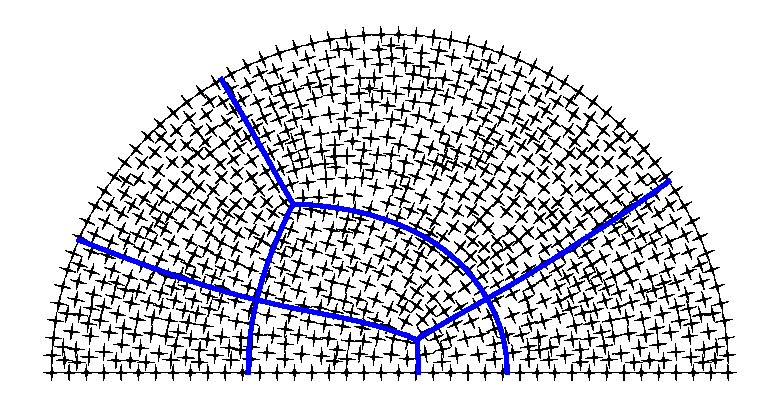
\includegraphics[scale=0.32]{images/demiDiscGinzAligne.eps}\\\vspace{0.1cm}
    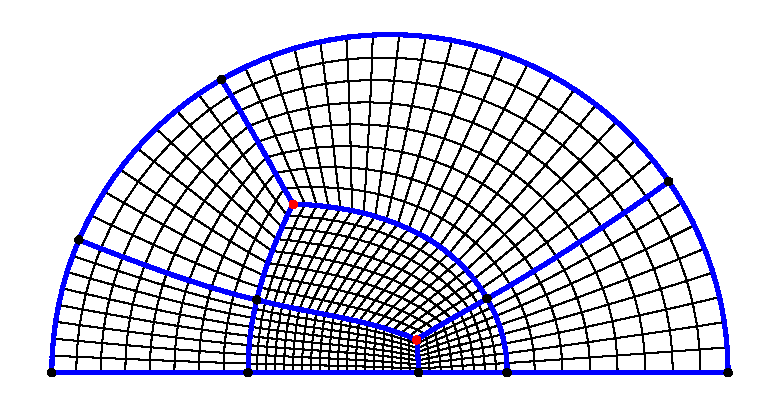
\includegraphics[scale=0.32]{images/demiDiscMail.eps.eps}\\
    \scriptsize {\color{onera_gray}(Champ analytique)}
\end{column}
\pause
\begin{column}{0.4\textwidth}
    \centering
    \scriptsize
    $\chi(\Omega)=1$\\\vspace{0.1cm}
    $deg(\bar{u}, \partial\Omega) = 1/4+1/4+1/4$\\\vspace{0.1cm}
    $\sum_{i=1}^{3} id_{\bar{u}}(c_i)=1/4+1/4-1/4$\\\vspace{0.1cm}
    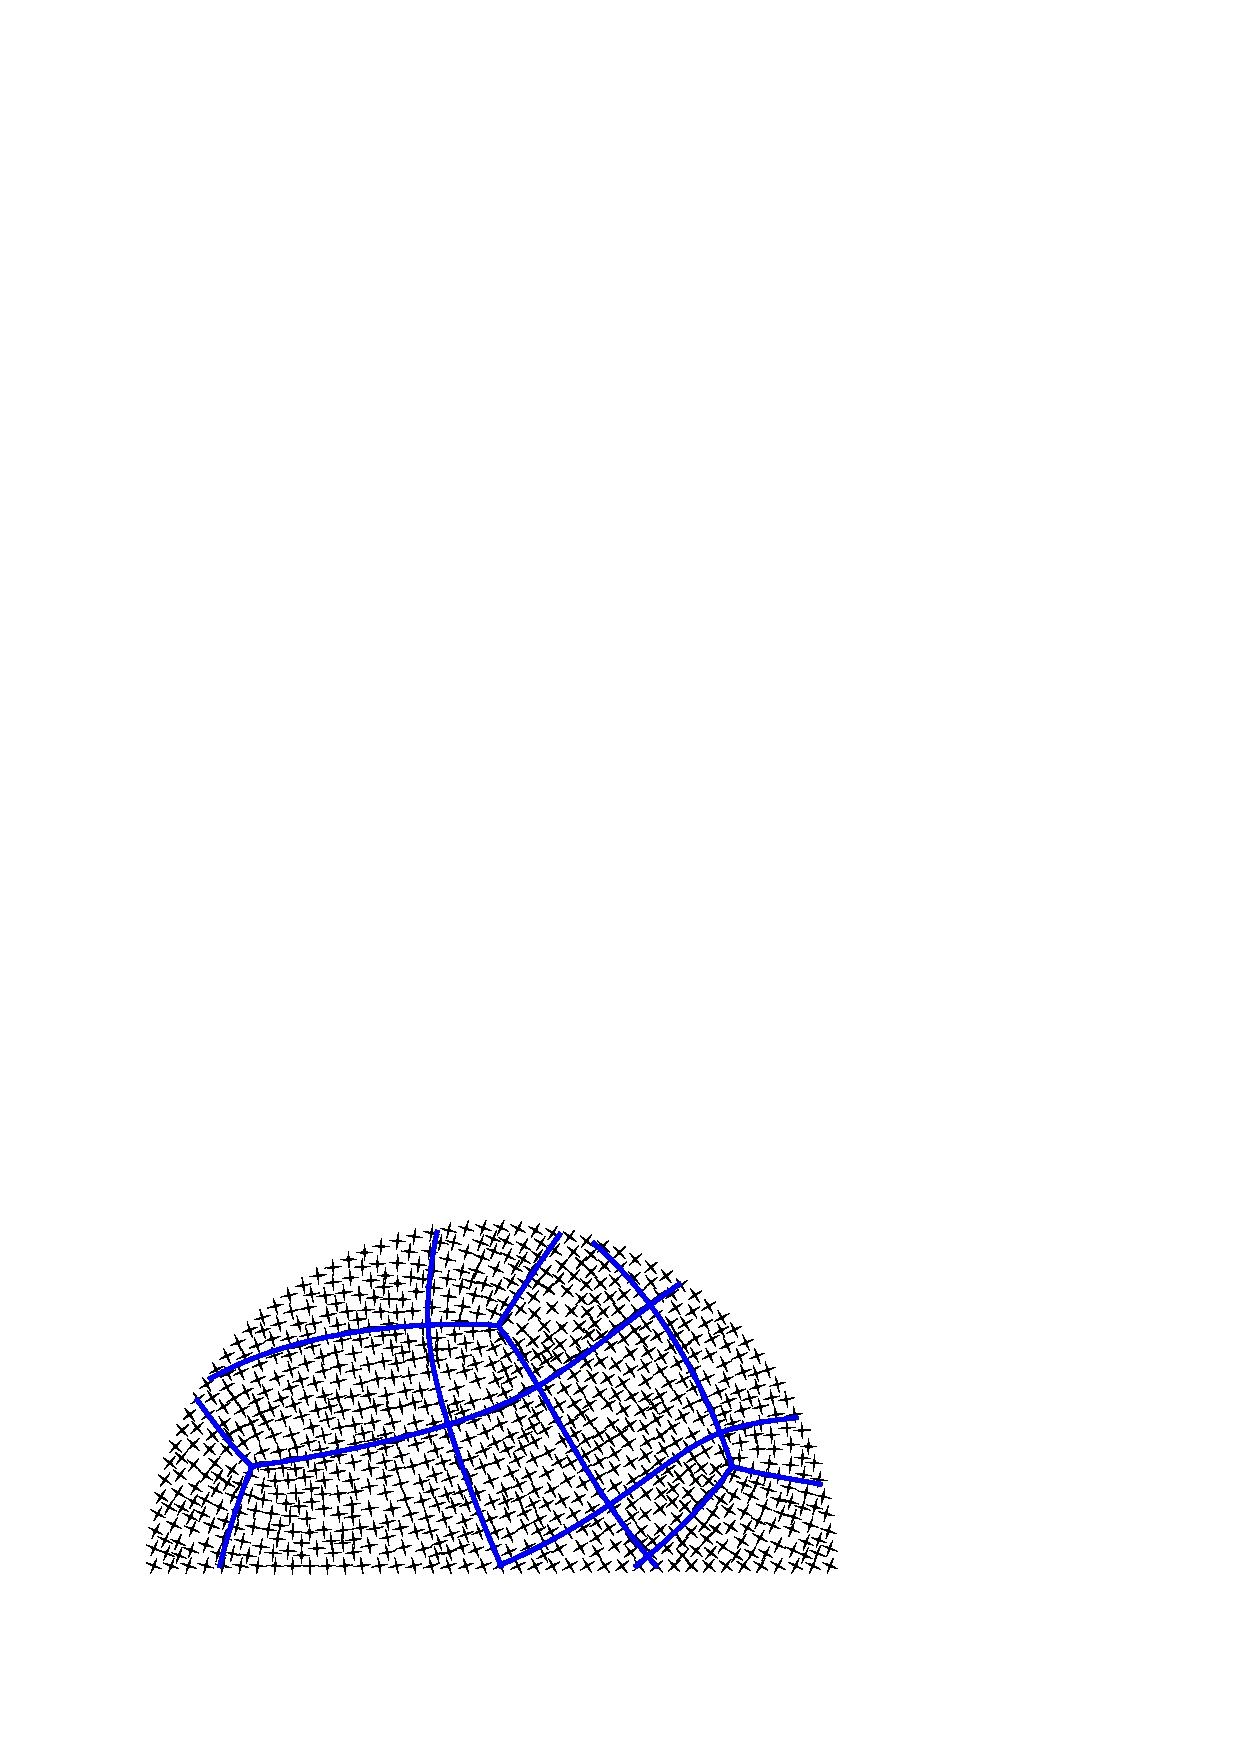
\includegraphics[scale=0.32]{images/demiDiscTroisPointNonAligne.pdf}\\\vspace{0.1cm}
    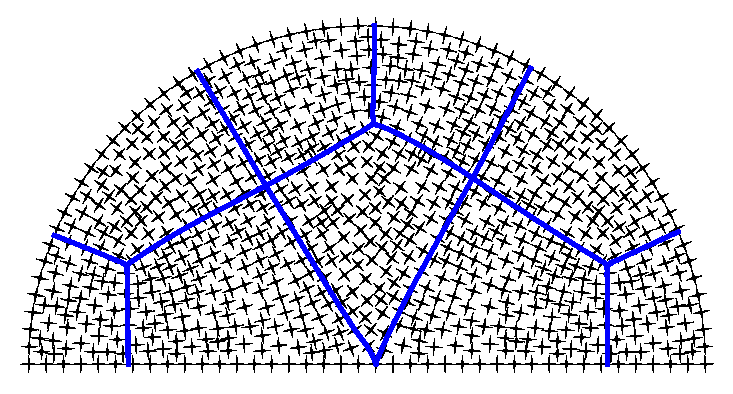
\includegraphics[scale=0.32]{images/demiDIscTroisPointAligne.eps}\\\vspace{0.1cm}
    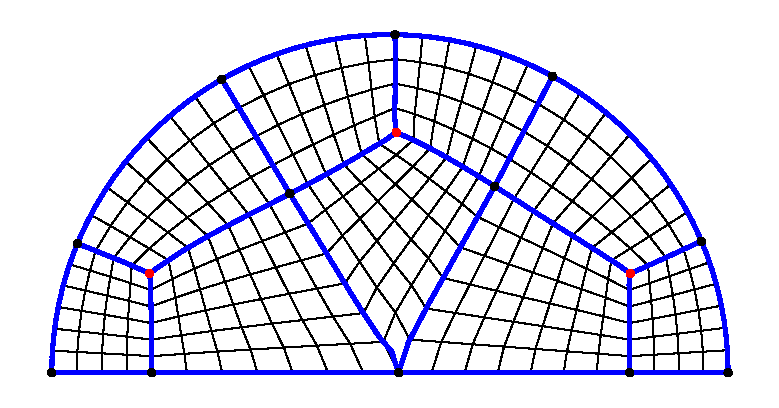
\includegraphics[scale=0.32]{images/mesh_quad_3.eps}\\
    \scriptsize {\color{onera_gray}(bonus pts. sing. bord, vue coin.)}
\end{column}
\end{columns}
\end{frame}


\begin{frame}{Travaux de recherche}
\small
{\bf Bilan}\\\vspace{0.2cm}
\begin{itemize}
\item Formalisation de la notion de champ de croix, plusieurs définitions (index, angle, rotation, ...)\\\vspace{0.1cm}
\item Mise en évidence des conditions nécessaires à l'obtention d'un maillage quadrilatéral à partir d'un champ de croix (Théorème 1)\\\vspace{0.1cm}
\item Mise en place du processus d'alignement (Théorème 2)\\\vspace{0.1cm}
\item Introduction des points singuliers de bord\\\vspace{0.2cm}
\end{itemize}
{\bf Plus loin}\\\vspace{0.2cm}
\begin{itemize}
\item Extension aux domaines non simplement connexes et gestion des multimatriaux (Théorème 3)\\\vspace{0.1cm}
{\color{onera_gray}\small Détail, (Domaine qui ne peuvent être continuellement réduit à un point, typiquement d'un seul tenant avec plusieurs bords, domaines à trous)}, {\color{onera_gray} Echec du processus d'alignement. Non régularité du champ dû à la non-périodicité de la différence des croix sur les bords}
\end{itemize}
\end{frame}



\begin{frame}{Travaux de recherche}{Domaines non-simplement connexes}
%\vspace{-0.1cm}
\small
\begin{columns}
\begin{column}{0.68\textwidth}
Construction d'un champ de correction vérifiant l'équation faible:%\\\vspace{0.1cm}
\begin{equation*}
\left\{
\begin{array}{lcll}
    \triangle h &= &0 &\mbox{ dans }\Omega,\\[0.025cm]
    \displaystyle\frac{1}{2\pi}\int_{\Gamma_0}\theta_h &=& deg(\bar{u}, \Gamma_0)-1+\sum_j id_{\bar{u}}(b_j^0))&\mbox{ sur } \Gamma_0,\\[0.025cm]
    \displaystyle\frac{1}{2\pi}\int_{\Gamma_i}\theta_h& =& deg(\bar{u}, \Gamma_i)-1-\sum_j id_{\bar{u}}(b_j^i),&\mbox{ sur }\Gamma_i~~~\forall~i.
\end{array}
\right.
\end{equation*}
Champ de croix finale {\color{onera_gray} (obtenue via une double rotation, champ cor., champ align.)}
\begin{equation*}
\bar{v}=R(\phi)R(\theta_h)\bar{u}.
\end{equation*}
%\textbf{Exemple:} Application au carré troué.\\\vspace{0.2cm}
\begin{onerablock}[drop fuzzy shadow]{
\small Théorème 3}
\'Etant $\bar{u}$ donné un ensemble $(c_i)_{i\in\{1,\dots,n_b\}}\subset\partial\Omega$ de points distincts tel que:
$
{\bf deg(\bar{u}, \partial\Omega) = \chi(\Omega)-\sum_{i=1}^{n_b} id_{\bar{u}}(c_i),}
$
le champ de croix $\bar{v}=R(\phi)R(\theta_h)\bar{u}$ vérifie le Théorème 1.
\end{onerablock}
\end{column}
\begin{column}{0.32\textwidth}
\centering
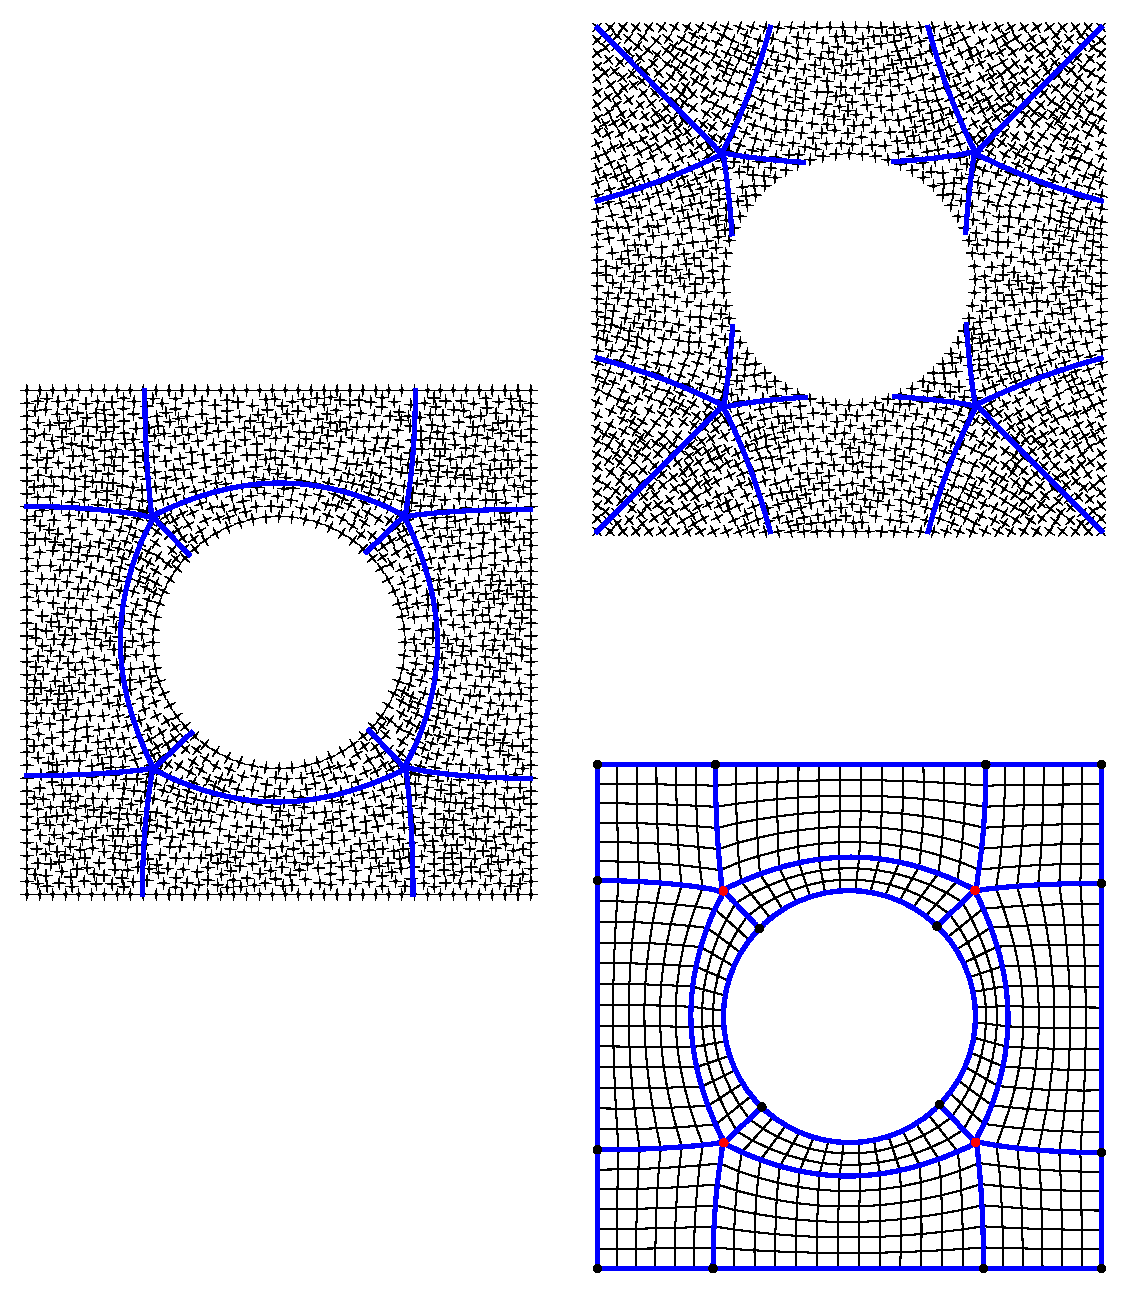
\includegraphics[scale=0.27]{images/image.eps}
\end{column}
\end{columns}
\end{frame}




\begin{frame}{Travaux de recherche}
\small
\vspace{-0.4cm}
{\bf Implémentation du processus de partitionnement sur un maillage triangulaires nous permettant de développer des algorihmes et méthodes à savoir:}%\\\vspace{0.2cm}
\begin{columns}
    \begin{column}{0.6\textwidth}
\begin{itemize}
\item Construction d'une représentation discrète du champ de croix\\%\vspace{0.1cm}
\item Approximation des séparatrices\\\vspace{0.1cm}
\item Traversé des triangles singuliers\\\vspace{0.1cm}
\item Paramétrisation des partitions\\\vspace{0.1cm}
\item Extension aux surfaces courbes\\\vspace{0.1cm}
\item Mise en place d'une librairie prototype HQMESH implémentant la méthode en C++.\\\vspace{0.3cm}
\end{itemize}
    \end{column}
    \begin{column}{0.4\textwidth}
        \centering
        \includegraphics[scale=0.28]{images/vagues.png}
    \end{column}
\end{columns}
Présentation détaillée aux JSO du projet JEROBOAM et du LMA2S le 08/07/2024.
\end{frame}



\begin{frame}{Travaux de recherche}
\small
\only<1>{
{\bf Publications}
\begin{itemize}
\item Kokou Dotse, Vincent Mouysset, Sébastien Pernet: \textit{Theoritical analysis of four sided partitioning of a planar surface from a cross field}, SIAM Journal on Scientific Computing (soumis).\\\vspace{0.2cm}
\item Kokou Dotse, Vincent Mouysset, Sébastien Pernet: \textit{Discrete Formulation of a Structured Quad-Block Mesh Generation Method from Cross Fields on 2D Manifolds} (en préparation).\\\vspace{0.2cm}
\item Kokou Dotse, Vincent Mouysset, Sébastien Pernet: \textit{Quadrilateral mesh of non-simply connected domain and non-planar surfaces from a given cross-field, The SIAM International Meshing Roundtable Workshop 2023} (proceeding).\\\vspace{0.2cm}
\item Rapport technique, Note d'avancement du PRF JEROBOAM - Année 2021 (année 2)- Année 2022 (année 3).\\\vspace{0.2cm}
\end{itemize}
}

\only<2>{
{\bf Communications}
\begin{itemize}
\item \textit{Quadrilateral mesh of non-simply connected domain and non-planar surfaces from a given cross-field}, The SIAM International Meshing Roundtable Workshop 2023 (SIAM IMR 2023), Amsterdam, Netherlands, 06-09 Mars 2023.\\\vspace{0.2cm}

\item \textit{Génération de maillages quadrilatéraux à partir de champs de croix donnés}, Journées Ondes du Sud-Ouest 2023 (JOSO 2023), Toulouse, France, 14-16 Mars 2023.\\\vspace{0.2cm}

\item \textit{Quadrilateral mesh create from a given cross field}, 10th International Conference on Curves and Surfaces, Arcachon, France, 20-24 Juin 2022.\\\vspace{0.2cm}

\item \textit{Méthode de maillage en quadrilatères par résolution d’EDP}, Laboratoire de Mathématiques Appliquées à l’Aéronautique et au Spatial (LMA2S), Toulouse, France, Mars 2021.\\\vspace{0.2cm}

\item Journée des doctorants de l’ONERA, Châtillon, France, 01 Février 2022, 20 Janvier 2023.\\\vspace{0.2cm}
\end{itemize}
}
\end{frame}


\begin{frame}{Plan}
%\tableofcontents
\vspace{-0.4cm}
\begin{enumerate}
\color{onera}
\item {\color{onera_gray}Cursus et expériences professionnelles}\\\vspace{0.5cm}
\item {\color{onera_gray}Travaux de recherche} \\\vspace{0.5cm}
\item {\color{onera}Projet de recherche et intégration dans les activités de MACI/ONERA} {\color{onera_gray} \small (construit dans un désir d'interactions et d'utilisation pour les schémas numériques (coeur des activités MACI, s'inscrit naturellement dans certains axes du LMA2S), par rapport à des activité déjà en cour dans l'équipe ou qui pourrait être mise en place.)}\\\vspace{0.5cm}
\item {\color{onera_gray}Conclusion}
\end{enumerate}
\end{frame}



\begin{frame}{\large Projet de recherche et intégration dans les activités de MACI/ONERA}{Retour sur le problème de l'homogénéisation}
\small
Rappel: Notre méthode de gestion de l'homogénéisation consiste à choisir un champ de croix adapté. Important pour les problématiques de CFL.\\\vspace{0.2cm}
{\bf Commment gérer automatiquement le positionnement des points singuliers dans le processus d'homogénéisation?}\\\vspace{0.2cm}
\begin{itemize}
    \item reperer des zones d'équilibre dans le domaines et y placer les points singuliers
    \item deplacement des points du maillage sans perdre la connectivité (Ex: lissage laplacien)\\\vspace{0.2cm}
\end{itemize}
\begin{columns}
    \begin{column}{0.55\textwidth}
\centering
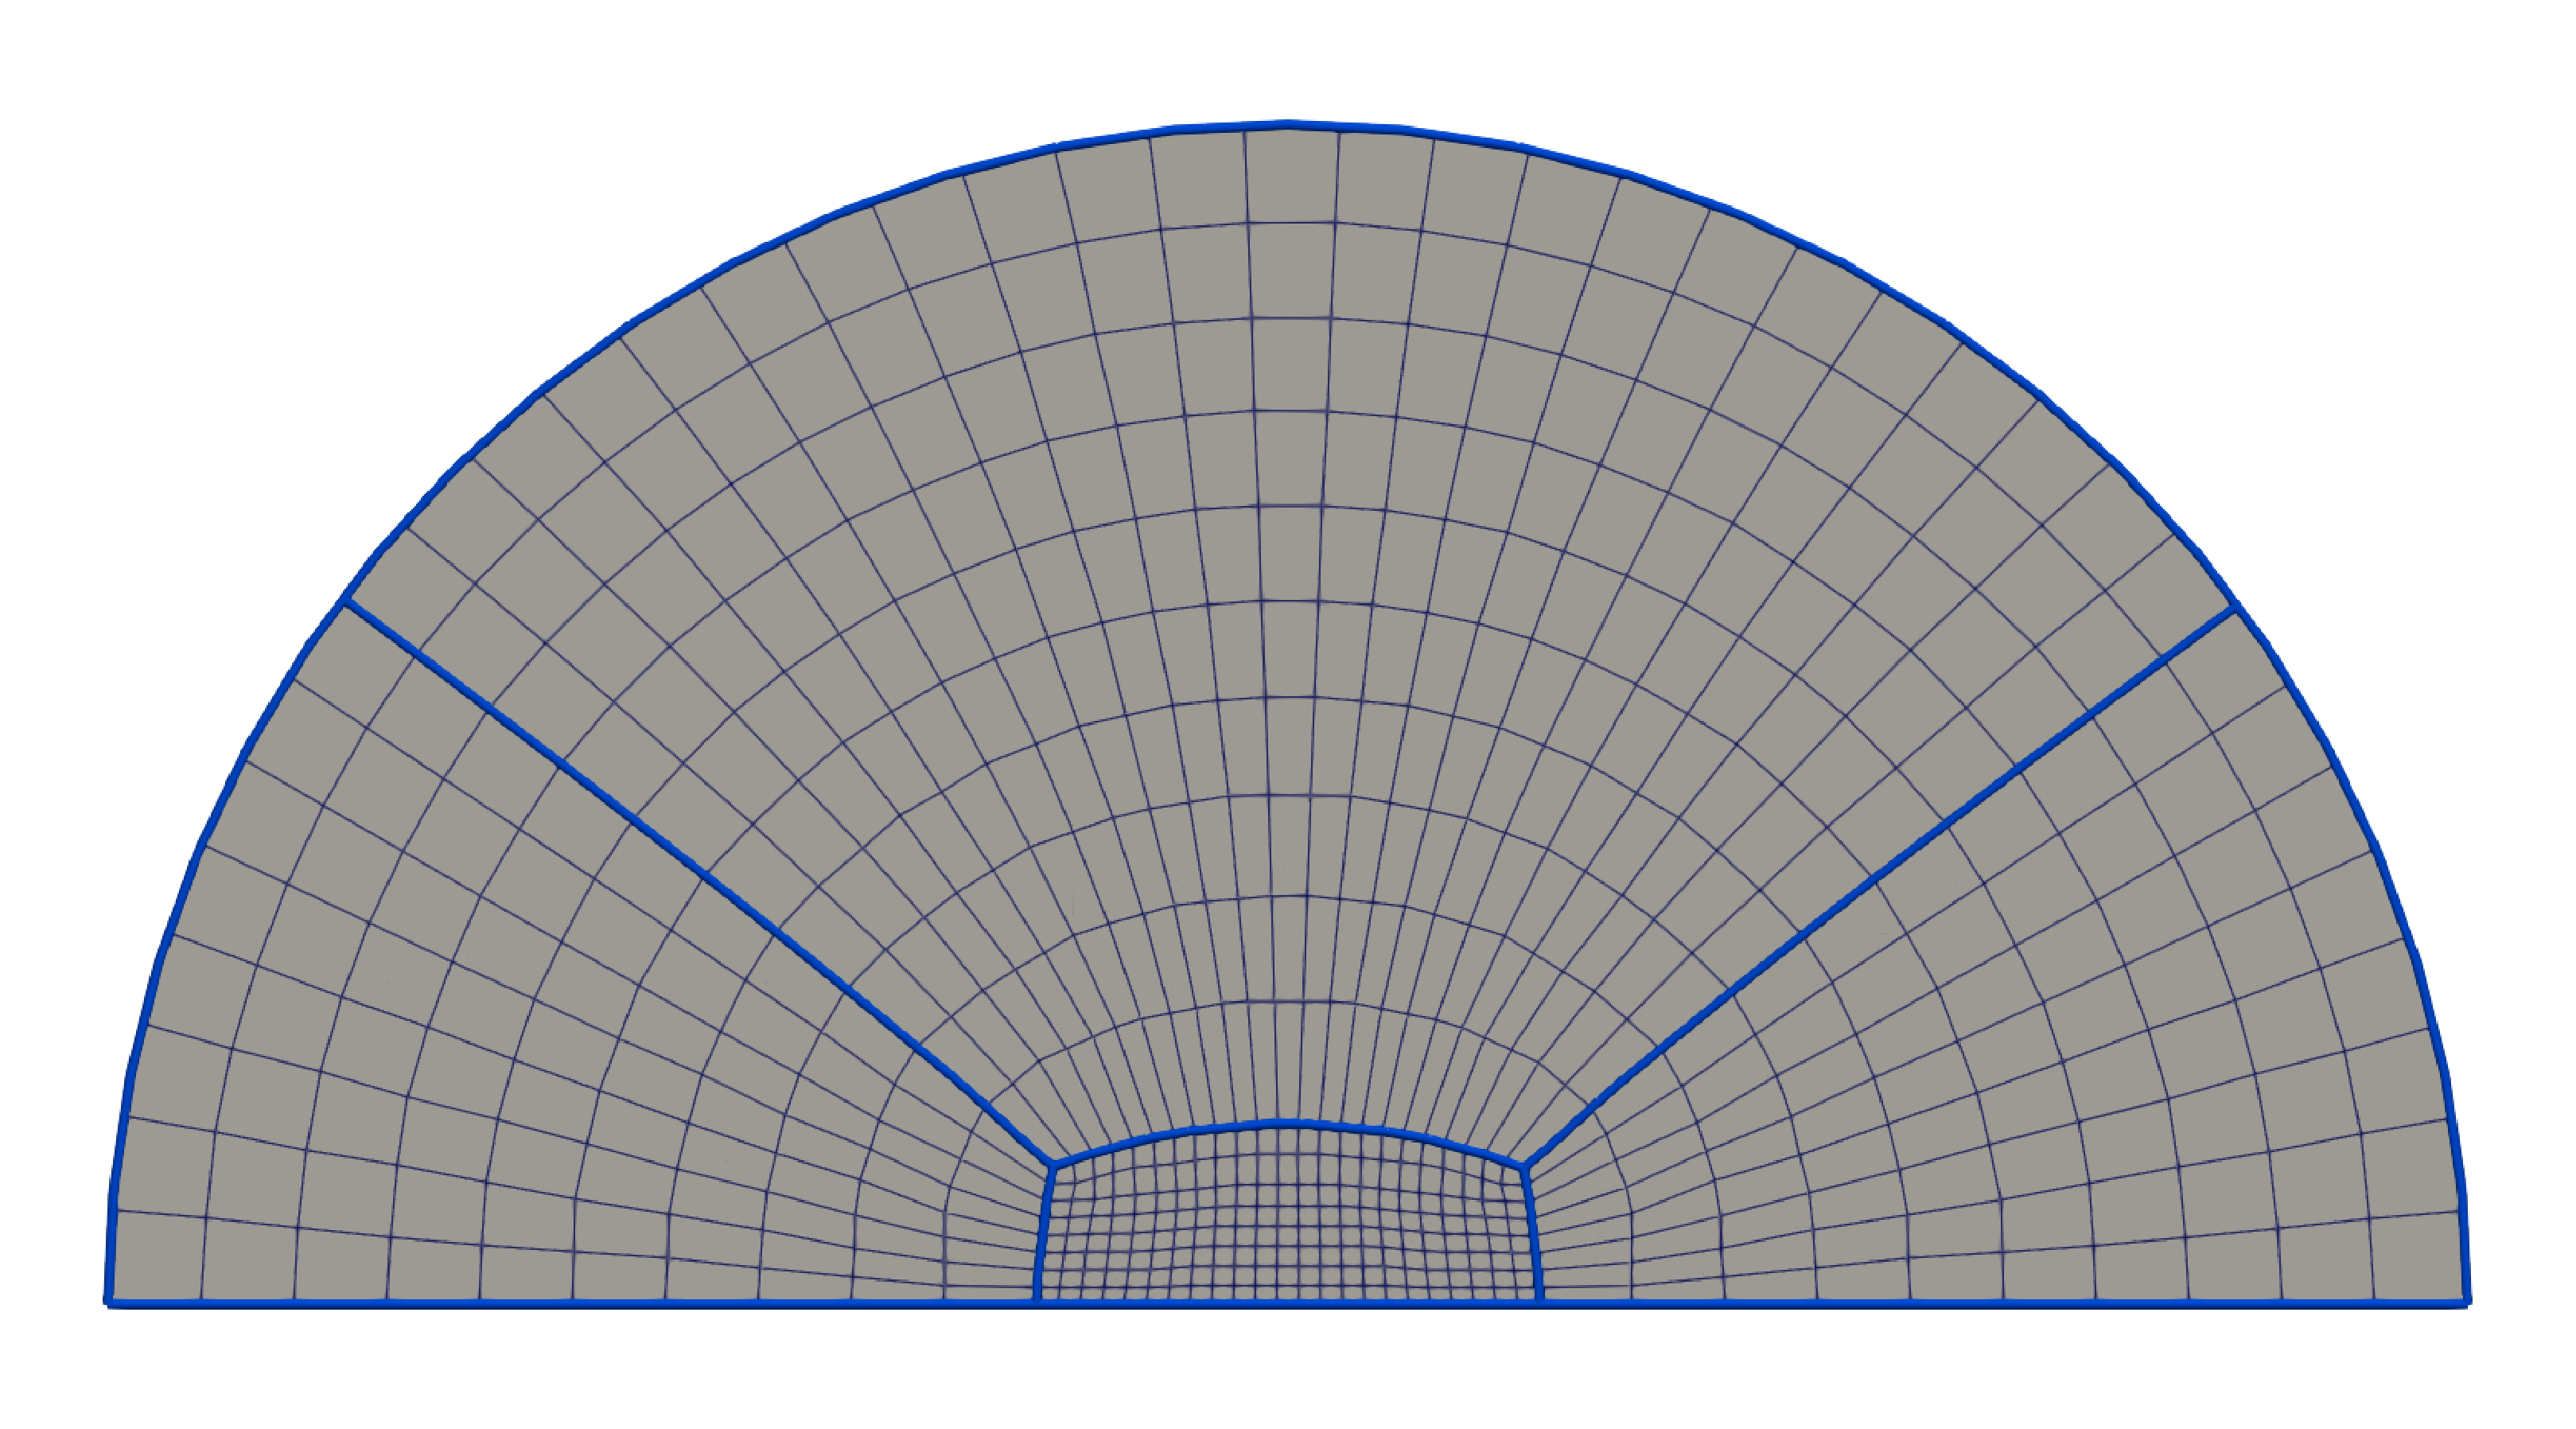
\includegraphics[scale=0.09]{images/non_homo_demiDisc.pdf}\\
\footnotesize Non-homogène
    \end{column}
    \begin{column}{0.55\textwidth}
        \centering
\includegraphics[scale=0.09]{images/homo_avec_bord_demiDisc.pdf}\\
\footnotesize Homogène (OCV)
    \end{column}
\end{columns}
\end{frame}



\begin{frame}{\large Projet de recherche et intégration dans les activités de MACI/ONERA}{Pourrais t'on adapter le partitionnement?}

%\begin{columns}
%    \begin{column}{0.55\textwidth}
%\centering
%\includegraphics[scale=0.1]{images/rect_demi_disc_first.pdf}
%\hspace{0.1cm}
%\includegraphics[scale=0.1]{images/rect_demi_disc_second.pdf}
%    \end{column}
%    \begin{column}{0.55\textwidth}
%        \centering
\small
Par exemple dans le cadre d'un remaillage remaillage avec une estimation a posteriori ou pour avoir un maillage guidé par une quantité physique.\\\vspace{0.3cm}
Idée: Proposer un champ de croix aligné le plus possible sur une référence (d’angle $\theta$) et respectant des contraintes issues d’un autre champ de croix (d’angle $\phi$). Ce qui reviendrait à remplacer l'équation d'alignement par le problème de minimisation suivant:\\\vspace{0.3cm}

\begin{equation*}
\begin{cases}
    \tilde{\theta} := \theta + \alpha\phi \in C^1(\Omega), \\
    \min_{\substack{\alpha=1 \\ \partial\Omega}} \left\lvert \theta - \tilde{\theta} \right\rvert,
\end{cases}
\end{equation*}
$$
\alpha^* = \arg\min_{\alpha\in C^1(\Omega,[0,1]), \alpha=1 \text{ sur } \partial\Omega} \left( \lVert \alpha\phi \rVert_\infty + \lambda \lVert \nabla (\alpha\phi) \rVert_\infty \right).
$$
%\end{column}
%\end{columns}
\end{frame}



\begin{frame}{\large Projet de recherche et intégration dans les activités de MACI/ONERA}{Comment gérer les cycles limites ?}
\small
\vspace{-0.5cm}
\begin{center}
\includegraphics[scale=0.15]{images/cycle_limit_1.pdf}\hspace{0.8cm}
\includegraphics[scale=0.15]{images/cycle_limit_2.pdf}
\end{center}
%\vspace{0.3cm}
\textbf{Rappel} : Les cycles limites sont exclus dans les résultats présentés.\\\vspace{0.1cm}
Les cycles limites apparaissent lorsque les séparatrices ne convergent pas. Exemple (voir figure).\\\vspace{0.1cm}
\textbf{Comment gérer les cycles limites ?} Une idée serait de stopper ces séparatrices et de regarder les systèmes de partitionnement de type Catmull-Clark.
%\begin{columns}
%\begin{column}{0.6\textwidth}
%\centering
%Illustration avec un cycle limite
%\end{column}
%\begin{column}{0.5\textwidth}
%\centering
%\includegraphics[scale=0.1]{images/limit_cycle_1.pdf}
%\hspace{0.1cm}
%\includegraphics[scale=0.1]{images/limit_cycle_2.pdf}\\
%\scriptsize Premier cas.\\
%\includegraphics[scale=0.1]{images/limit_cycle_3.pdf}
%\hspace{0.1cm}
%\includegraphics[scale=0.1]{images/limit_cycle_4.pdf}\\
%\scriptsize Deuxième cas.\\
%\includegraphics[scale=0.1]{images/limit_cycle_5.pdf}
%\hspace{0.1cm}
%\includegraphics[scale=0.1]{images/limit_cycle_6.pdf}\\
%\scriptsize Troisième cas.\\\vspace{0.4cm}
%\end{column}
%\end{columns}
\end{frame}



\begin{frame}{\large Projet de recherche et intégration dans les activités de MACI/ONERA}{Qu'en ait'il des domaines périodiques ?}
\small
\begin{columns}
    \begin{column}{0.55\textwidth}
Problème de simulation physique qui requiert des conditions de bord periodique. Exemple du LS89 (Voir figure)\\\vspace{0.3cm}

\textbf{Problème:} Les partitions ne sont pas alignés ce qui induit une perte d'efficacité du fait de ne pas pouvoir exploiter les avantages des blocs structurer (on pourrait interpoler les données mais cela couterait beaucoup plus cher)\\\vspace{0.3cm}

\textbf{Idée:} Construire le champ de croix de tel sorte que les points d'entrées et de sorties des séparatrices appartiennent à une même ligne de niveau.

%ce qu'on aimerait que les points d'entrée soit les points de sortie.\\\vspace{0.3cm} Une idée est que c'est point appartiennent à une même ligne de niveau.

%les points singuliers d'index 0 pourraient permettre d'integrer des séparatrices à

%les decoupages de zones doivent etre periodique

%points de sortie comme points d'entrée (risque de cycle limite, augmentation du nombre de partitions)

%streamline creer par integration d'edp
%si le champ est periodique cela ne resoud pas le problemes

%par construction le champ de croix est periodique car geometrie periodique, normal periodique, champ de croix periodique.

%ce qu'on aimerait que les points d'entrée soit les points de sortie. Une idée est que c'est point appartiennent à une même ligne de niveau.

%placé a et b sur le Dessin
    \end{column}
    \begin{column}{0.45\textwidth}
    \vspace{-0.5cm}
        \centering
\includegraphics[scale=0.22]{images/LS89_transparent.png}
%\\\footnesize Superposition du maillage du LS89.
    \end{column}
\end{columns}
\end{frame}


% \begin{frame}{\large Projet de recherche et intégration dans les activités de MACI/ONERA}{Reconstruction du bord du domaine}
% \small
% Rappelons que le candidat de champ de croix que l'on construit est régulier à cause de la procédure d'alignement et converge vers une solution régulière. On pourrait donc :\\\vspace{0.3cm}
%     \begin{itemize}
% \item Faire de la reconstruction de gradients de bord\\\vspace{0.3cm}
% \item Mettre en place un processus de reconstruction de courbure locale maille par maille.\\\vspace{0.3cm}
% \item Un stage est actuellement en cours à l'ONERA dans l'équipe MACI sur ce sujet.
%     \end{itemize}
% \end{frame}




\begin{frame}{\large Projet de recherche et intégration dans les activités de MACI/ONERA}%{Reconstruction du bord du domaine}
\small
%\begin{itemize}
%\item
{\color{onera}Mise en oeuvre d'applications les maillages quadrilatéraux:}  évaluation des performances en aéroacoustique, et en particulier par l'utilisation de maillages d'ordres élevés (Activité proposé par Vincent Mouysset avec Christophe peyret (DAAA/NFLU)).\\\vspace{1cm}
%\item
{\color{onera}Extension de la méthode aux domaines volumiques:} (3D, Maillage hexaédrique, besoin certain), développement d'un caddre théorique similaire à ce qui est fait en 2D plan et en surfacique, développer des méthodes d'hybridation entre tétraèdre et hexaèdre bloc-structuré. (Activité proposé par Vincent Mouysset avec  Xavier ferrieres (DEMR/CME)).\\\vspace{0.2cm}
%\end{itemize}
\end{frame}


\begin{frame}{\large Projet de recherche et intégration dans les activités de MACI/ONERA}
\small
\vspace{-0.18cm}
Lors de ma thèse, sujet assez varié, géométrie numérique, géométrie différentiel et riemanniennnee, analyse d'EDP, programmation avancée, calcul parallèle, C++, python , OpenMP.\\
Confiance et désir de m'ouvrir à encore plus de sujets et de défis, tant sur le plan mathématique que numérique.\\\vspace{0.1cm}
\begin{itemize}
\item {\color{onera} Modèle Multi-échelles et Multi-Physiques:} décharges plasma, modèle fluide d'essaims de drône, mobilité urbaine (Guillaume Dufour).\\\vspace{0.1cm}
\item {\color{onera} Optimisation:} modèles de substitution par réseaux de neuronnes (Patricia Klotz).\\\vspace{0.1cm}
\end{itemize}
Très interesser par les interactions entre les schémas numériques et le machine learning.\\\vspace{0.1cm}
\begin{itemize}
\item {\color{onera} Amélioration de la résolution numérique de certaines EDP en termes d’approximations d’ordre élevé :} piste explorée par Guillaume Dufour et Sébastien Pernet.\\\vspace{0.1cm}
\item {\color{onera} Régression par processus gaussien :} recherches par Eric Savin.\\\vspace{0.1cm}
\end{itemize}
Plus généralement, je m'intéresse aux projets de développement logiciel mettant en lumière les algorithmes et méthodes implémentés dans le cadre des travaux de l'équipe.\\\vspace{0.1cm}
\end{frame}




\begin{frame}{Conclusion}
\small
{\bf Pourquoi intégrer l'ONERA et plus spécifiquement l'équipe MACI?}\\\vspace{0.5cm}
\begin{itemize}
\item {\color{onera} Acteur majeur de la recherche aéronautique et spatiale en France :} au cœur de pôles d’innovations scientifiques et technologiques de grande envergure à travers toute la France avec des problématiques réelles permettant d'orienter des recherches mathématiques théoriques comme appliquées.\\\vspace{0.5cm}
\item {\color{onera} Mon passage dans l'équipe MACI pour ma thèse :} garantit d'être intégré dans une équipe avec laquelle je partagerai ma passion tout en restant autonome et avec des responsabilités qui pourraient m'être rapidement confiées.\\\vspace{0.5cm}
\item {\color{onera} Enseignement :} possibilité de dispenser un enseignement en université et en école.
\end{itemize}
\end{frame}


%%%%%%%%%%%%%%%%%%%
% Page de remerciements (optionnel) %
%%%%%%%%%%%%%%%%%%%
\ThankYouFrame{Merci de votre attention!}
%\\\vspace{10pt}Des questions ?}

%%%%%%%%%%%%%%
%Bibliographie (optionnel) %
%%%%%%%%%%%%%%
%\ReferencesFrames{./biblioJDD}
\end{document}
